\documentclass[12pt, a4paper]{ctexart}

% 页面与排版设置
\usepackage[margin=2.54cm]{geometry}
\usepackage{amsmath, amssymb}
\usepackage{booktabs}
\usepackage{graphicx}
\usepackage{float}
\usepackage{color}
\usepackage{xcolor}
\usepackage{array} 
\usepackage[colorlinks=true, linkcolor=black, urlcolor=blue, citecolor=black]{hyperref}
\usepackage{enumitem}           % 支持 enumerate 的 label= 参数

% 全局容差设置，彻底修复 Underfull / Overfull \hbox 警告
\setlength{\emergencystretch}{5em}
\tolerance=10000

% ---------- 字体与伪粗体设置 ----------
\usepackage{fontspec}
\setmainfont{Times New Roman} % 英文要求使用 Times New Roman

% 解决 macOS 字体找不到粗体产生的警告
\xeCJKsetup{AutoFakeBold=true}
\setCJKmainfont[AutoFakeBold=true]{Songti SC}      % 宋体
\setCJKsansfont[AutoFakeBold=true]{Heiti SC}       % 黑体
\setCJKmonofont[AutoFakeBold=true]{STFangsong}     % 仿宋

% ==========================================
% 全局中文标题样式设置 (严格遵循作业要求的“第X部分”格式)
% ==========================================
\ctexset{
    section = {
        format = \centering\zihao{3}\heiti, % 1级标题：黑体3号字居中
        name = {第,部分},                       
        aftername = {：},                   % 冒号分隔，例如：第一部分：从辐射光到数字
        number = \chinese{section},         
    },
    subsection = {
        format = \raggedright\zihao{-3}\heiti, % 2级标题：黑体小3号字左对齐
        name = {},                       
        number = \arabic{section}.\arabic{subsection}, % 阿拉伯数字编号，如：1.1
    },
    subsubsection = {
        format = \raggedright\zihao{4}\heiti, % 3级标题：黑体4号字左对齐
        name = {},
        number = \arabic{section}.\arabic{subsection}.\arabic{subsubsection}, % 阿拉伯数字编号，如：1.1.1
    }
}

% 修复目录中 section 级别没有点点点的问题，包括摘要
\makeatletter
\renewcommand{\l@section}{\@dottedtocline{1}{0em}{1.5em}}
\makeatother

% 页眉页脚设置 (删除上方标题和页码，改为右下方)
\usepackage{fancyhdr}
\pagestyle{fancy}
\fancyhf{} % 清空所有的页眉和页脚
\renewcommand{\headrulewidth}{0pt} % 删除页眉的横线
\rfoot{\thepage} % 将页码放置在右下角

% 兼容 ctextart 自动调用 plain 样式的特殊页面（如目录首页）
\fancypagestyle{plain}{
    \fancyhf{}
    \renewcommand{\headrulewidth}{0pt}
    \rfoot{\thepage}
}

% 代码高亮设置
\usepackage{listings}
\definecolor{codegreen}{rgb}{0,0.6,0}
\definecolor{codegray}{rgb}{0.5,0.5,0.5}
\definecolor{codepurple}{rgb}{0.58,0,0.82}
\definecolor{backcolour}{rgb}{0.96,0.96,0.96}

\lstdefinestyle{pystyle}{
    backgroundcolor=\color{backcolour},   
    commentstyle=\color{codegreen},
    keywordstyle=\color{magenta},
    numberstyle=\tiny\color{codegray},
    stringstyle=\color{codepurple},
    basicstyle=\ttfamily\small,
    breakatwhitespace=false,         
    breaklines=true,                 
    captionpos=b,                    
    keepspaces=true,                 
    numbers=left,                    
    numbersep=5pt,                  
    showspaces=false,                
    showstringspaces=false,
    showtabs=false,       
    tabsize=4
}
\lstset{style=pystyle}

% ---------- 自定义上标引用命令 ----------
\newcommand{\scite}[1]{\textsuperscript{[#1]}}

\begin{document}

% ==========================================
% 自定义封面页
% ==========================================
\begin{titlepage}
\begin{center}
    ~\\[10.5pt]
    \textbf{\songti\zihao{1}  北京电影学院课程作业}
    ~\\[10.5pt] ~\\[10.5pt] ~\\[10.5pt] ~\\[10.5pt]

    {\zihao{2}\bfseries 数字影像捕获与再现技术\\专题研究报告}
    
    ~\\[10.5pt] ~\\[10.5pt] ~\\[10.5pt] ~\\[10.5pt]
    ~\\[10.5pt] ~\\[10.5pt] ~\\[10.5pt] ~\\[10.5pt]
    ~\\[10.5pt] 
    
    \begin{tabular}{>{\heiti\fontsize{16pt}{16pt}\selectfont}r>{\kaishu\fontsize{16pt}{16pt}\bfseries\selectfont}l}
        作　　者：    &   祝庆\\[4pt]
        院　　系：    &   智能影像工程学院\\[4pt]
        专　　业：    &   影视技术\\[4pt]
        教学层次：    &   本科生\\[4pt]
        年　　级：    &   2023 级\\[4pt]
        学　　号：    &   231112014\\[4pt]
        指导教师：    &   顾晓娟 \hspace{0.5em} 鲁梦河\\[4pt]
        成　　绩：    &   \\[4pt]
        日　　期：    &   2026 年 5 月\\[4pt]
    \end{tabular}

\end{center}
\end{titlepage}

% ==========================================
% 前置部分（使用罗马数字页码：Ⅰ, Ⅱ, Ⅲ...）
% ==========================================
\newpage
\pagenumbering{Roman} % 设置页码为大写罗马数字并从1开始

% ==========================================
% 中文摘要（单独一页）
% ==========================================
\phantomsection
\addcontentsline{toc}{section}{中文摘要} % 将中文摘要手动加入目录
\begin{center}
    {\heiti\zihao{3} 内容摘要} % 项目名称用3号黑体字
\end{center}
\vspace{1em}
{\fangsong\zihao{-4} % 内容用小4号仿宋体字
\setlength{\parindent}{2em} % 起首空两格
本报告系统梳理了数字影像从场景辐射光到最终数字码值所经历的光电转换、信号处理、色彩还原及新型显示适配技术的完整链路。报告首先阐释了光子到电子、模拟到数字的物理数学基础，对比了专业电影摄影机与智能手机计算摄影在系统工程上的根本分歧；随后深度解析了光电转换函数（OETF）的数学本质及其在专业影视与移动端设备上的差异化设计；进而梳理了从传统统计方法到人工智能、多光谱传感器等白平衡方案的技术跃迁；最后重点探讨了 Lofic 横向溢出积分电容与 Gain Map（增益映射）两项突破性技术，深度解构了 Gain Map 的底层数学模型与色彩保真机制，并揭示了其在跨设备自适应显示中的核心价值，以及从 Adobe/Google 私有方案到 ISO 21496-1 国际标准的标准化演进路径。全文力求在保持学术严谨性的同时，以通俗的类比和直观的分析，帮助读者建立起对现代数字影像技术体系的整体认知。\par
}

% 利用 vfill 将关键词推至页面底部
\vfill
% 关键词用4号黑体字，不超过5个以空格区隔
\noindent {\heiti\zihao{4} 关键词：数字影像\quad 光电转换函数\quad 白平衡\quad Gain\ Map\quad 计算摄影}

% ==========================================
% 英文摘要（单独一页）
% ==========================================
\newpage
\phantomsection
\addcontentsline{toc}{section}{Abstract} % 将英文摘要手动加入目录
\begin{center}
    {\zihao{3}\textbf{Abstract}} % 项目名称用3号 Times New Roman
\end{center}
\vspace{1em}
{\zihao{-4} % 内容用小4号 Times New Roman
\setlength{\parindent}{2em}
This report systematically sorts out the complete pipeline of digital imaging from scene radiance to final digital values, covering photoelectric conversion, signal processing, color reproduction, and new display adaptation technologies. It first explains the physical and mathematical foundations from photons to electrons and from analog to digital, and compares the fundamental differences between professional cinema cameras and smartphone computational photography in systems engineering. Then, it provides an in-depth analysis of the mathematical nature of the Opto-Electronic Transfer Function (OETF) and its differentiated design in professional film and mobile devices. Subsequently, it reviews the technological leap in white balance solutions from traditional statistical methods to artificial intelligence and multi-spectral sensors. Finally, it focuses on two breakthrough technologies—Lofic lateral overflow integration capacitor and Gain Map. It deeply deconstructs the underlying mathematical model and color fidelity mechanism of Gain Map, and reveals its core value in cross-device adaptive display, as well as the standardization path from Adobe/Google proprietary schemes to the ISO 21496-1 international standard.\par
}

\vfill
% 英文关键词用4号 Times New Roman，排印在本页下端
\noindent {\zihao{4}\textbf{Key words:}\quad digital imaging\quad OETF\quad white balance\quad Gain Map\quad computational photography}

% ==========================================
% 目录
% ==========================================
\newpage
\phantomsection
\addcontentsline{toc}{section}{目录} % 将目录自身也加入到目录列表
\renewcommand{\contentsname}{\centering\heiti\zihao{3} 目\quad 录}
\tableofcontents


% ==========================================
% 正文开始（使用阿拉伯数字页码，且格式为 01, 02...）
% ==========================================
\newpage
\pagenumbering{arabic} % 页码切换回阿拉伯数字并重置为1
\renewcommand{\thepage}{\ifnum\value{page}<10 0\arabic{page}\else\arabic{page}\fi} % 小于10前面补0

\section{从辐射光到数字}

\subsection{场景辐射光到数字码值的完整处理流程}

数字影像的核心本质，是将现实世界中连续的物理光辐射能量，通过跨越光学、固态半导体物理与数字信号处理等多个学科的复杂管线，转换为离散的数字矩阵。无论是院线级专业电影摄影机还是高度集成化的智能手机，从“场景辐射光（Radiance）”到最终输出的“数字码值（Digital Value）”，均需要经历一套严密的光电转换数学与物理流程。

这一处理流程的起点是辐射度与光学投影阶段。现实场景中的辐射度通常表示为关于空间位置和波长的连续函数，在经过摄像机镜头的光学折射与透射后，投射到传感器焦平面上形成辐照度（Irradiance）。在此物理过程中，镜头的光学孔径、透过率（T-stop）以及边缘渐晕效应直接决定了到达传感器的光子通量密度。如果把单颗像素比作一只收集雨水的小桶，那么镜头口径就是桶口的大小，而快门时间则是收集的时长。桶中积蓄的“水量”，就是辐照度在曝光时间内的积分——这便是曝光量。

随后进入光电转换与电荷积累阶段。焦平面上的互补金属氧化物半导体（CMOS）传感器利用光电效应，通过光电二极管将到达的物理光子转化为电子并储存在势阱中。由于光子到达时间的不确定性与量子波动特性，这一光电转换过程严格受泊松分布支配，从而从底层引入了不可避免的光子散粒噪声。传感器的量子效率决定了光子转化为电子的绝对转换率，而满阱容量则决定了像素在达到物理饱和前所能容纳的最大电子数，这直接框定了单次曝光下的物理动态范围上限。直观理解，大像素就像大水桶，能装更多的“电子雨水”，因此即便光线微弱也不容易干涸（噪声低）；小像素则相反，一点点的光子涨落就足以淹没信号。

积累在像素势阱中的电子随后进入模拟信号放大与模数转换阶段。电子被读出电路转化为微弱的模拟电压信号，通过可变增益放大器（其物理对应于相机的原生 ISO 或增益设置）进行信号放大。经过放大的模拟电压被送入模数转换器（ADC）进行空间与幅度的双重量化，输出原始的数字码值。在这一关键的转换节点，系统会不可避免地引入读出噪声和暗电流噪声。整个物理到数字的转换模型可以被高度数学化地概括为：记录的数字码值等于光子通量积分、散粒噪声、模拟增益与读出噪声的综合函数结果，并受限于 ADC 的最大量化阈值。

最终，由 ADC 输出的拜耳阵列原始数据被送入图像信号处理器（ISP）进行计算与编码。这一数字处理管线包含了大量的非线性运算，核心步骤包括：黑电平扣除以校正暗电流基准、坏点消除、通过去马赛克算法恢复全采样 RGB 图像、色彩空间转换矩阵映射、白平衡校正以及空域和时域的降噪处理。在管线的末端，ISP 会应用光电转换函数（OETF），将呈线性分布的数字信号压缩为非线性的数字码值，以符合人类视觉系统对对数亮度的感知特性，并大幅优化存储与传输的比特率分配。整个流程就像把自然界的光线经过一系列“翻译”和“包装”，最终变成显示屏上可见的像素。

\begin{table}[H]
\centering
\caption{从辐射光到数字码值的关键转换节点}
% 使用 raggedright 修复可能会产生的 Underfull 警告
\begin{tabular}{@{} >{\raggedright\arraybackslash}p{3cm} >{\raggedright\arraybackslash}p{6cm} >{\raggedright\arraybackslash}p{5cm} @{}}
\toprule
\textbf{处理阶段} & \textbf{物理/数学过程} & \textbf{主要噪声/误差来源} \\ \midrule
光学投影          & $E = \int L \cdot \mathrm{d}\Omega$（辐照度积分） & 渐晕、杂散光 \\
光电转换          & 光子 → 电子（量子效率） & 光子散粒噪声 \\
电荷积累          & 电子储存在势阱中 & 满阱容量限制 \\
模拟放大与 ADC     & 电压放大 + 离散化量化 & 读出噪声、暗电流噪声、量化误差 \\
ISP 数字处理       & 去马赛克、色彩校正、降噪、OETF 压缩 & 算法伪影、比特深度限制 \\ \bottomrule
\end{tabular}
\end{table}

\subsection{专业摄影机与智能手机的流程异同与硬件特点分析}

尽管光子到电子的基础量子物理原理完全一致，专业电影摄影机（如 ARRI ALEXA、RED、Sony CineAlta 系列）与智能手机计算摄影系统在截然不同的应用场景驱动下，其系统工程设计与硬件权衡呈现出巨大的分歧。一个通俗的比喻可以说明：专业摄影机如同装备精良的科研实验室，拥有宽敞的空间和精密的仪器，追求在控制条件下获得最纯粹、最丰富的数据；而智能手机则像一个随身携带的智能助手，必须在极度受限的体积和功耗条件下，依靠实时计算“脑补”出令人满意的结果。这种差异体现在传感器的每一个角落。

表 \ref{tab:comparison} 从多个维度梳理了二者的核心差异。

\begin{table}[H]
\centering
\caption{专业电影摄影机与智能手机系统差异对比}
\label{tab:comparison}
\renewcommand{\arraystretch}{1.3}
% 加入了 >{\raggedright\arraybackslash} 强制左对齐，彻底修复原本严重的 Overfull / Underfull \hbox 报错
\begin{tabular}{@{} >{\raggedright\arraybackslash}p{2.8cm} >{\raggedright\arraybackslash}p{6cm} >{\raggedright\arraybackslash}p{6cm} @{}}
\toprule
\textbf{对比维度} & \textbf{专业电影摄影机（ARRI ALEXA 35）} & \textbf{智能手机计算摄影（旗舰机型）} \\ \midrule
核心场景与目标 & 
院线级电影工业、受控布光、严苛后期调色，追求极致光学宽容度与物理光线还原。 & 
即时社交分享、复杂混合光照，追求“按下快门即出片”与便携性。 \\ \addlinespace
传感器尺寸 & 
Super 35 至全画幅，物理面积 > 800 mm²，巨大的受光面积带来极高的光子收集能力。 & 
1/2.8 至 1 英寸，物理面积 30–110 mm²，受限于机身厚度，进光量严重不足。 \\ \addlinespace
像素尺寸与信噪比 & 
像素 > 6 µm，满阱容量极大，原生暗部噪声极低，可单帧捕获 17 档动态范围。 & 
像素 1.0–1.6 µm，即便采用四合一技术，满阱容量依然受限，暗部噪点明显。 \\ \addlinespace
光学系统 & 
可换镜头、物理光圈精确控制、T-stop 标定，可通过机械手段控制景深和通光量。 & 
固定微型镜头、超大固定光圈（f/1.6 以上），缺乏物理光圈调节，依赖计算景深模拟。 \\ \addlinespace
ISP 机制 & 
\textbf{光学本真捕获}：单帧超高动态范围 RAW/Log，极少量 ISP 干预，将创作权完全留给后期。 & 
\textbf{强计算摄影}：多帧合成、AI 降噪、局部色调映射，输出高度加工的图像和视频，旨在弥补物理硬件的不足。 \\ \bottomrule
\end{tabular}
\end{table}

深入探究这两种系统的分歧可以发现，手机与专业摄影机在“从辐射光到数字”链路上的核心冲突在于对“信噪比与动态范围的获取方式”的根本差异。专业摄影机依靠巨大的硅片面积，在“空间维度”一次性收集海量光子，从而建立了无懈可击的原生信噪比基础。而手机受制于物理体积，不得不转向“时间维度”（多帧积分）与“算法维度”（深度学习降噪与语义重建）来代偿。这种高度复杂的非线性融合管线，虽然能在静态或低速场景下输出惊人画质，但在拍摄高速运动物体或复杂混合光源时，也极易产生时序错位导致的重影伪影和过度锐化带来的“计算痕迹”。例如，用手机拍摄夜间的旋转摩天轮，轮辐边缘常常出现鬼影，这就是多帧合成算法在时空对齐失败后的典型表现。

\section{OETF（光电转换函数）的深度解析}

\subsection{OETF与EOTF的定义及其在影像系统中的核心作用}

在现代色彩科学与视频工程体系中，传递函数是连接物理光辐射、数字比特流与人类视觉神经感知的核心桥梁。影像数据的存储与传输带宽极其昂贵，传递函数的存在使得工程师能够以最高效的方式对光线进行编码与解码。

在我们日常的视觉经验中，人眼对光线的感受并非线性。在昏暗的房间里，一根蜡烛的点燃会带来巨大的亮度变化感知；而在阳光明媚的户外，同样数量的光子增加，我们却几乎察觉不到。这正是韦伯-费希纳定律所描述的现象：人类视觉系统的亮度感知近似对数特性，对暗部极其敏感，对高光相对迟钝。

然而，影像传感器却是高度线性的器件——它每接收一个光子，就忠实地产生一个电子。如果我们将这种线性信号直接量化为数字码值，就会出现严重的资源错配：大量珍贵的比特被浪费在人眼根本无法分辨的极端高光区域，而人眼最为敏感的暗部区域，却因量化精度不足而出现明显的色阶断层（Banding）。这就像一个只有 100 个刻度的尺子，却要同时测量毫米级的高度变化和千米级的距离，结果必然顾此失彼。

为了解决这一矛盾，工程师们在摄像机的信号处理管线中插入了光电转换函数（OETF）。从数学角度看，OETF 的本质是一个非线性压缩器：它将传感器输出的庞大线性光信号，映射为符合人眼感知特性的非线性数字电信号。如此一来，有限的量化位深（如 10-bit 的 1024 个灰阶）便能重新分配，向暗部和中间调倾斜更多的数据位，从而在有限的存储和传输带宽下，最大限度地抑制暗部色带现象。

在显示端，电光转换函数（EOTF）负责将传输过来的非线性视频信号解码，并转换为屏幕上实际发射的线性显示光。需要注意的是，OETF 与 EOTF 并非简单的数学互逆关系。系统的端到端特性被称为光光转换函数（OOTF），它是 OETF 与 EOTF 的级联。由于观众所处的室内观影环境通常比拍摄现场暗得多，人眼对对比度的感知会发生漂移，因此 OOTF 通常被设计为具有略大于 1.0 的系统伽马（如 1.2），以在较暗的环境中重塑接近现场感受的视觉对比度。这意味着，OETF 的设计师必须前瞻性地考虑目标显示设备的 EOTF 特性和预期观看环境，二者共同协作才能将导演的艺术意图准确地传递给观众。

\subsection{OETF转换技术的发展历程}

影像传递函数的演进史，是一部不断与存储带宽限制和显示介质物理特性博弈的编年史。我们可以将其大致划分为四个阶段：

\begin{enumerate}[label=\textbf{阶段 \arabic*：}]
    \item \textbf{线性阶段}：早期数字视觉系统直接保留信号与光子数之间的线性关系。这种编码方式极其浪费资源，大量比特分配给肉眼难以分辨的极端高光，而暗部却因量化不足而呈现严重断层，就好比用 100 块钱买 1 粒米，却只花 1 块钱买一袋面。
    \item \textbf{CRT 补偿 Gamma 阶段（如 BT.601 / BT.709）}：在标准动态范围（SDR）电视时代，阴极射线管（CRT）显示器的电子枪本身具有约 2.4 次幂的非线性电光响应。为了在模拟传输中补偿这一缺陷，摄像机端引入了约 0.45 次幂的 OETF 进行预校正。这一物理层面的工程妥协，巧合地高度匹配了人眼的暗部敏感特性，使得仅有 8-bit 的 SDR 信号在全球范围内大规模普及并沿用至今。我们今天在普通电视和网页上看到的绝大多数图像，依然基于这一曲线的变种。
    \item \textbf{对数曲线时代（Logarithmic / Cineon）}：随着数字电影摄影机的动态范围突破 14 档，传统的 BT.709 曲线已无法容纳如此宏大的光影跨度。电影工业借鉴传统胶片的密度响应特性，引入了对数编码。其核心逻辑是：将曝光档位的倍增，转化为数字码值的等量增加。也就是说，每增加一档光圈，码值就增加相同的幅度。这种平坦、去饱和化的“数字底片”极大保留了高光和暗部的极限细节，为后期调色提供了无比宽广的操作空间，但也因此显得“灰蒙蒙”，必须经过专业的色彩校正才能恢复悦目的画面。
    \item \textbf{高动态范围（HDR）时代（HLG / PQ，ITU-R BT.2100）}：为了支持 1000 尼特甚至更高的现实 HDR 显示，国际电联确立了两种新传输函数。PQ（Perceptual Quantizer，感知量化）彻底抛弃相对亮度概念，基于人眼 Barten 对比度敏感度模型，是一种绝对亮度编码，可精确映射从极暗到 10000 尼特的物理亮度，是杜比视界等格式的基础\scite{1}\scite{2}。HLG（Hybrid Log-Gamma，混合对数伽马）则采用折中设计：下半部分沿用传统 Gamma 曲线以兼容旧有 SDR 显示器，高光部分平滑过渡为对数曲线，从而无需动态元数据即可实现广播级的 HDR 直播与分发\scite{1}。
\end{enumerate}

\subsection{不同设备的EOTF/OETF分类与特点剖析}

\subsubsection{专业电影摄影机 OETF 设计哲学}

专业电影机的 Log 曲线无一例外地被设计为“场景参考（Scene-Referred）”，其唯一使命就是以最高保真度封装传感器捕获的极限动态范围，为后期色彩科学提供最纯净的数学基底。它们不负责“好看”，只负责“完整”。

\begin{itemize}
    \item \textbf{ARRI LogC4：恒定斜率与曝光指数独立性} \\
    LogC4 是 ARRI 为其 ALEV4 传感器量身定制的第四代对数编码，配合更为宽广的 ARRI Wide Gamut 4 (AWG4) 色彩空间使用。它最具革命性的特点是实现了曝光指数（EI）的绝对独立性——无论摄影师如何更改 ISO 设定，硬件编码曲线的“伽马”斜率保持恒定，仅发生整体信号的线性位移。这使得 17 档动态范围内的每一档曝光都能获得均匀且精确的量化步长，彻底杜绝了高光或暗部的数据挤压，也使得后期数字解码管线大为简化。ARRI 为此专门发布了 LogC4 与 ARRI Wide Gamut 4 白皮书，系统阐述了这一对数编码的数学基础与设计哲学\scite{3}。ARRI REVEAL 色彩科学团队宣称，这一对数设计使最终影像在数学响应上最逼近人类视网膜的生物学情感响应\scite{4}。
    \item \textbf{Sony S-Log3：致敬 Cineon 的纯粹对数容器} \\
    Sony 的 S-Log3 曲线形状高度致敬了经典的 Cineon 数字底片规格。它移除了高光区的肩部压限，压平了暗部的趾部，使线性对数段极长。S-Log3 在 18\% 中性灰的色调下实现了约 1.5 档的动态范围扩展，整体有效宽容度可达约 15.3 档\scite{5}。作为一种极其纯粹的对数编码，S-Log3 不在机内对极端高光做任何主观的滚降妥协，为调色师提供了无限接近传感器物理极限的“原材料”。
    \item \textbf{RED IPP2 体系下的 Log3G10：为极端色彩保留容器} \\
    RED 的 Log3G10 曲线将 18\% 中性灰精确映射到全信号范围的 1/3 处，并极为夸张地保留了在中性灰之上编码 10 档动态范围的能力\scite{6}。其核心哲学是“技术控制与创意渲染的绝对解耦”。极为宽广的 Log3G10 容器与 REDWideGamutRGB 色域，旨在防止拍摄极端高亮度且高饱和色彩（如 LED 霓虹灯、警车尾灯）时经常出现的色域溢出与色相扭曲，将高光滚降和色调映射完全后置到输出转换阶段，由调色师自由裁量。
\end{itemize}

\subsubsection{智能手机计算摄影 OETF 设计逻辑}

随着移动端算力的井喷与杜比视界等 HDR 格式的普及，旗舰智能手机也开始引入自有的对数曲线。但由于物理底层的根本性掣肘，其 OETF 呈现出极具妥协性与计算辅助性的特殊设计。

\begin{itemize}
    \item \textbf{Apple Log：抛物线趾部与暗部噪声的巧妙编码} \\
    苹果在 iPhone 15 Pro 及后续机型的 ProRes 录制中引入了专属的 Apple Log\scite{7}。引人瞩目的是，Apple Log 的高光和中间调部分呈现标准的对数分布，但在极暗部区域（趾部），该曲线并没有像传统电影机那样进行平缓的对数延伸，而是数学上平滑地过渡为一个\textbf{抛物线（Parabola）}。这一设计的根本原因在于移动端小尺寸传感器的本底噪声极大。如果生硬地套用纯对数曲线，在暗部极低的亮度水平下，传感器由于信噪比崩溃而产生的极其微弱的信号波动甚至“负电压波动”，会在对数解算时被无限放大，产生灾难性的彩噪。苹果设计的抛物线趾部允许系统在进行 10-bit 数字捕获时，有效且平滑地编码“负信号”，从而保留了底层噪声的真实统计学分布特性，使得 iOS 内置 ISP 或后期软件中的空域降噪算法能够更精确地剥离底层噪声，而不至于破坏暗部的实际色彩细节。这本质上是一种“先诚实地记录噪声，再聪明地去除它”的策略。
    \item \textbf{OPPO O-Log：在小底与10-bit容器之间艰难博弈} \\
    OPPO 推出的 O-Log 采用一种相对标准的对数函数模型 $P = \gamma \cdot \ln(R+\beta) + \delta$，配合等同于 BT.2020 的 O-Gamut 广色域。由于移动端硬件编码器的限制，其实际落地依托于 10-bit H.265 (HEVC) 有损编码压缩（4K 60fps 码率约 120 Mbps）。O-Log 的核心价值在于，在 ISP 管线极早期就将 14-bit 高动态原始线性数据，无损地非线性重映射并压缩进有限的 10-bit 容器中。这是一种在存储带宽、传感器面积与极宽广的自然光照之间艰难博弈的系统工程选择。
\end{itemize}

\subsection{手机与摄影机OETF设计之间的核心差异及原因}

为什么智能手机不能且不应该直接套用 ARRI LogC4 或 Sony S-Log3 曲线？这需要从硅基半导体物理学、信息论量化精度与计算摄影理念三个维度进行剖析：

\begin{enumerate}
    \item \textbf{物理像素面积与信噪比的不可逾越之壁} \\
    专业摄影机的单像素面积可达手机的 10 倍以上，满阱电子容量海量，原生暗部信噪比极高，能够真正“看清”阴影中的光学细节。电影机的 Log 曲线被设计为均匀覆盖 17 档的宏大动态范围。然而，智能手机传感器的真实物理宽容度可能仅有 10 到 12 档。如果手机强行套用 ARRI 的 LogC4 曲线，由于曲线跨度极大，大量宝贵的数字码值会被强行分配给手机传感器根本无法捕获到的“超高光”和“超深暗部”（这些区域在手机上传感器上只有饱和死白和纯粹的热噪声）。这会导致真正含有有效信息的中间调被严重压缩，信噪比进一步恶化，最终整个画面充满粗糙的散粒噪声，且毫无层次可言。
    \item \textbf{量化位深与色阶断层效应的冲突} \\
    为了支撑其极端的对数压缩，专业电影机管线毫无例外地采用 12-bit 或 16-bit 线性/对数 RAW 作为数据载体，提供 4096 甚至 65536 个离散灰阶。而受限于移动端闪存的写入带宽与处理器的发热限制，智能手机（包括 iPhone 15 Pro 的 Apple Log）在进行视频录制时，硬件编码器的最高支持上限通常被锁定在 10-bit HEVC/ProRes（仅有 1024 级灰阶）。一个狭窄的 10-bit 容器根本无法承受如 S-Log3 那样激进陡峭的对数压缩，一旦强行套用，在天空、肤色等平滑色彩渐变区域，将不可避免地产生毁灭性的色阶断层现象。
    \item \textbf{对计算摄影干预程度的本质妥协} \\
    电影机 Log 的终极存在意义是提供未经任何粉饰的原始光学数据。但手机的感光元件过于孱弱，它必须时刻依赖 ISP 进行极为强力的多帧时域降噪（MFNR）、空域滤波与多帧融合来续命。手机的 OETF（例如 Apple Log 具有抛物线性质的暗部趾部）正是为了辅助并兼容其底层复杂的计算降噪算法而特意扭曲设计的，这是追求纯粹线性光学响应的电影摄影机所绝不需要考虑的设计维度。
\end{enumerate}

通俗地说，电影机 Log 曲线是一条宽广笔直的高速公路，专为大马力跑车（高信噪比传感器）而建；手机若贸然驶入，只会因动力不足（信噪比低）而频繁熄火，且狭窄的车厢（10-bit）根本无法装载沿途的所有风景。因此，手机必须设计一条符合自身条件的专用道路，即使它看起来有些蜿蜒。

\section{色彩还原 —— 白平衡方案分析与对比}

在不同物理温度和属性的环境光源照射下，同一物体的反射光谱功率分布会发生剧烈变化。摄像机传感器必须具备消除环境光源色偏、将画面颜色精确重置回基准中性白（通常为 D65 标准光源）的能力，这一过程即为白平衡。自动白平衡是相机成像管线中至关重要的模块，其校正的准确性直接影响照片的视觉质量与下游计算机视觉任务的表现\scite{8}。随着底层算力的爆炸式增长与传感器技术的微型化，现代影像管线中的白平衡方案经历了从底层统计学、向人工智能深水区，再向多光谱物理测量方案的全面跃迁。

\subsection{传统统计学与底层启发式方案}

这一类方法基于对大自然宏观色彩分布的经验假设。最著名的是“灰世界假设”（Gray World），该算法假设一个拥有丰富色彩的自然场景中，所有像素颜色的平均反射值应该趋近于中立的灰色；系统据此计算出画面的全局颜色偏移并反向施加增益补偿。另一种常见的是“完美反射体/白点法”（White Patch / Max-RGB），其假设画面中最亮且未过曝的像素点即为场景中的绝对白色参考点。

\textbf{优势}在于算法复杂度极低，几乎不占用处理器算力，能够实现极低的延迟，并且极其容易在最廉价的 ISP 芯片底层硬件中实现硬化计算。
\textbf{致命缺陷}则是鲁棒性极度脆弱。由于算法本质是“盲目猜测”，一旦画面构图中被大面积的强烈单色物体占据（例如广袤无垠的纯蓝天空、一大片红色的砖墙），即触发“Color Wash”现象，算法就会不可避免地将这种正常的场景色彩误判为光源的色温偏移。这会导致系统做出方向完全错误的增益补偿，将壮丽的暖橘色夕阳强行修正为苍白，或是让站在红色背景前的人像肤色呈现诡异的青蓝色发绀。因此，这类方案仅适用于色彩分布均匀、包含明显白色参考物、纹理复杂且光源构成单一的常规全景户外摄影环境。

\subsection{基于深度学习与人工智能的白平衡方案}

为了克服传统方法在大面积纯色和混合光源下的误判，研究者们引入了深层卷积神经网络（CNN）或多层感知机（MLP）等 AI 模型\scite{9}。这些网络通过学习海量的真实场景数据，能够提取空域、色度乃至语义特征（例如识别出画面中的人脸、天空、草地），从而实现智能化的光源推断。

AI 方案从根本上降维打击了传统算法在纯色干扰下的尴尬局面。它不仅能通过语义分割识别出画面主体，智能分离并推断复杂的混合光源，还能对肤色这一人类视觉极度敏感的“记忆色”进行精准的局部色度保护与主观美学重构。例如，当画面中同时出现窗外的日光和室内的暖色台灯时，AI 白平衡可以尝试对画面进行空间可变的校正，使肤色保持自然，同时保留环境灯光营造的氛围感。最新的研究进一步提出利用智能手机的时间戳和地理位置等上下文元数据辅助光源估计，使 AWB 算法能够“知道此刻是日落”，从而避免将暖色调场景强行校正为中性白\scite{10}。在移动端，一些极轻量的色彩恒常性网络以不到 500 个参数便可在毫秒级完成高精度的光源推断，为实时视频白平衡提供了新的可能。

即便如此，AI 方案也非万能钥匙。其效果极度依赖训练数据集的质量与广度，神经网络本身的黑盒特性也使调试和归因变得困难。如果传感器在测试阶段遇到训练集中未曾覆盖的奇异人工光源（例如特定频段的工业 LED），算法可能发生灾难性的推断崩溃。此外，不同传感器之间的光谱响应曲线差异巨大，跨传感器部署往往需要耗费高昂成本重新收集数据集进行微调\scite{11}。目前，此类方案广泛部署于旗舰智能手机的多摄像头矩阵中，在复杂室内混合光源和人像拍摄场景下，已成为决定直出画质优劣的核心技术。

\subsection{基于多光谱传感器的硬件级白平衡方案}

这是从物理根源上解决色彩还原的最极端路径。它彻底抛弃纯粹基于 RGB 像素的软件推测，通过在设备上额外集成一枚独立的多通道光谱传感器（拥有 16 至 36 个窄波段通道），直接对入射光的光谱功率分布（SPD）进行“切片式”测量，从而在物理层面精确锁定环境光源独一无二的“光谱指纹”\scite{12}。每一类光源——无论是冷白 LED、暖白 LED 还是明亮日光——都具有其独特的 SPD 曲线特征，光谱传感器能够检测这一光谱签名，使相机精准识别光源类型并施以相应的白平衡校正\scite{12}。

这套方案最大的物理优势在于其无可挑剔的绝对精确性。它从原理上终结了“同色异谱”现象带来的误判烦恼——不论被摄物体的材质和背景色彩如何欺骗摄像头，系统都能提取出绝对准确的环境色温数据，并动态生成最匹配的色彩转换矩阵（CCM）。面对窗外 6500K 阳光与室内 2700K 暖光交织的极端混合光照场景，它可以提供完美的肤色还原以及极其精细的局部白平衡空间校正。Spectricity 公司已开发出世界上首款真正小型化、可量产的多光谱移动图像传感器 S1，为这一技术路线在消费电子领域的落地提供了可行路径\scite{13}。

当然，这种硬件级的方案会显著推高设备的物料成本（BOM），并在寸土寸金的机身背面额外占据开孔面积。同时，要求 ISP 引入全新的多维矩阵融合算法，使底层信号处理链路变得更加繁冗复杂。它最适合应用于对色彩要求极其苛刻的医疗皮肤诊断、精密工业检测、旗舰手机追求极限夜景混合光源拍摄，以及作为电影级外挂色温表，为最高规格的后期 DI 调色提供基准数据。

\section{拓展技术：Lofic技术与 Gain Map 探究}

在影像技术的演进中，如何将超越物理极限的光学宽容度捕捉到极小尺寸的硅片中，并如何在物理能力参差不齐的屏幕上完美重现这种宽容度，构成了影像系统两端的终极挑战。Lofic 与 Gain Map 这两项技术的出现，分别在捕获端与显示端引发了深刻的技术革命。

\subsection{Lofic技术}

Lofic（Lateral Overflow Integration Capacitor，横向溢出积分电容）是一种突破性的 CMOS 像素级硬件架构。在传统图像传感器中，由于像素面积有限，光电二极管在面对诸如直射太阳、强力车灯等极端强光时，电荷很快就会蓄满并发生饱和溢出，导致画面高光区域的细节与色彩完全丢失（即死白断层）。Lofic 技术创造性地在每一个微小像素的浮动扩散区旁边，巧妙地并联集成一个大容量的特殊电容。其物理机制犹如在容易溢出的水桶旁挖了一个巨大的水库：当光电二极管中的光生电子积累达到极限时，这些多余的电子并不会像废热一样被抛弃，而是“横向溢出”并被安全地储存在这个大电容中。

\textbf{优势与对 OETF 设计的影响}：在如 OmniVision 的 TheiaCel 技术或索尼 IMX908 等先进传感器中，Lofic 通常与双转换增益（DCG）技术结合使用\scite{14}。OmniVision 已在 2024 年正式发布采用 TheiaCel 技术的 OX03H10 图像传感器，该传感器利用单次曝光即可生成 140 dB 动态范围，并展现出无与伦比的 LED 闪烁抑制（LFM）性能\scite{14}。传感器在极暗处使用低读出噪声的高转换增益（HCG）读取信号，而在高光处则利用 Lofic 电容获取超大满阱容量的低转换增益（LCG），饱和电荷量可达到传统传感器的 20 倍。这种硬件级的内部缝合使得传感器能够在“单次极短曝光”下，直接输出高达 96 dB 甚至 110 dB 的恐怖动态范围。这对 OETF 设计提出了新的挑战：ISP 管线必须在执行对数压缩之前，进行极为精密的高低增益线性化拉平融合，否则两段曲线的物理拼接处会产生尖锐的数学“拐点”，导致后期出现不可逆的高光色带断层。

\textbf{与多帧合成 HDR 技术的对比分析}：完全摒弃了依赖不同曝光时长的多帧合成（Multi-frame HDR），Lofic 彻底从时间维度上消除了因物理时间差导致的运动重影伪影，也完美抑制了道路上 LED 交通灯或车辆尾灯由于脉冲调制带来的剧烈频闪（LED Flicker Mitigation, LFM）\scite{14}。而其\textbf{缺陷}在于，增加大容量物理电容不可避免地会侵占感光面积，若采用复杂的堆叠式设计又会显著推高芯片制造成本与功耗。

\textbf{如果传感器已经有了 Lofic 技术，我们还需要在软件层面开启 HDR 模式吗？}
答案是\textbf{绝对需要}。Lofic 在底层硅片上解决了极限宽容度的无损捕获，但这仅意味着 ISP “获取了极其充足且无过曝的原始数据”。智能手机仍然需要软件层面极具深度的计算摄影干预：首先，在弱光环境下，尽管不再有高光过曝危险，暗部的散粒噪声依然受限于微小的物理像素面积，必须通过时域多帧对齐融合来压制噪点；其次，如何将 Lofic 捕捉到的 110 dB 巨量线性数据，优雅地通过局部色调映射（Local Tone Mapping）重新压缩并塞进手机屏幕有限的显示动态范围中，这部分美学视觉重构依然完全仰仗计算 HDR 软件算法。

\subsection{Gain Map（增益映射）技术}

增益映射（Gain Map）的诞生重构了影像分发范式。它并非一种新格式，而是一种面向数字图像存储、跨设备传输与高动态显示渲染的革命性元数据编码架构。其核心哲学在于“相对编码”而非“绝对编码”：图像文件内不仅包含一张经过精心调色、适合在传统显示器上观看的基础图像（Base SDR，通常为 SDR 图像），还包含一张隐藏的、记录高光扩展比率的增益映射表以及一系列元数据\scite{15}。2025 年，国际标准化组织正式发布了 ISO 21496-1 标准，对增益映射及其关联元数据的定义、规格与使用方法做出了统一规范，标志着 Gain Map 技术从厂商私有方案走向了国际标准化的新阶段\scite{16}。当文件在不支持该技术的旧设备上打开时，直接显示基础 SDR 图像，实现完美的向后兼容；在支持 HDR 的环境中，渲染引擎则查询当前显示器的 HDR 头空间，动态插值并叠加增益，实时重构出完美适配屏幕物理极限的 HDR 图像。

\subsubsection{硬件限制与色彩偏移的物理根源}

\begin{figure}[H]
    \centering
    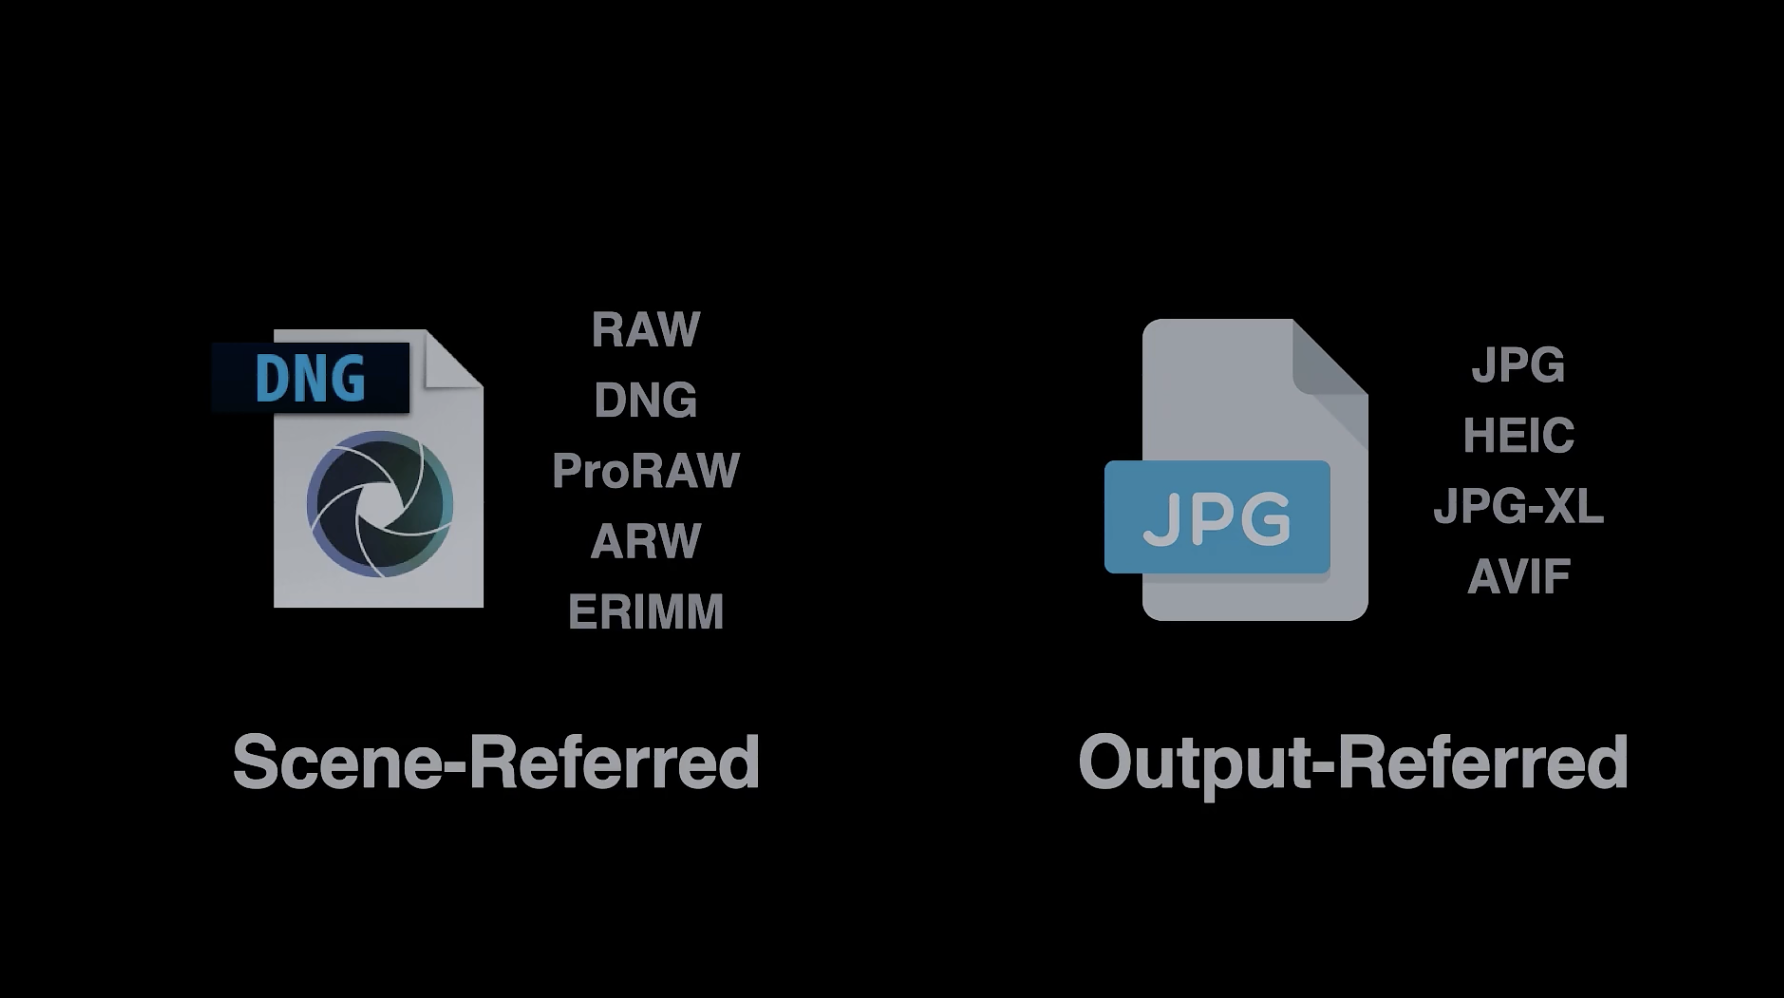
\includegraphics[width=0.65\textwidth]{gain_map_0.png}
    \caption{场景参考（RAW 等）与输出参考（JPG 等）的格式分类}
    \label{fig:scene_output}
\end{figure}

理解 Gain Map 特别是多通道彩色（RGB）映射的价值，需回溯至 CMOS 传感器的拜耳阵列物理机制。现代彩色相机在单色 CMOS 表面覆盖了 RGGB 拜耳滤色镜阵列，每个像素只能记录约三分之一的色彩信息，其余需通过去马赛克算法估算。在 HDR 场景中，面对极高亮度与高饱和光源（如红色霓虹灯），红色像素井会迅速饱和截断，而绿、蓝像素由于滤镜阻挡仍未饱和。当系统通过色调映射将这种极端动态范围压缩为 8-bit SDR 图像时，为避免大面积死白会强行压低整体亮度，导致原始的 R:G:B 能量比例被彻底破坏。最终在 SDR 中，纯正的红色会向补色偏移，呈现泛黄发白的颜色。这种由于物理限幅与不当色调映射引发的高光色相偏移与饱和度丢失，为 HDR 的后期重构带来了极大挑战。

\subsubsection{增益映射的对数空间数学模型（编码端）}

\begin{figure}[H]
    \centering
    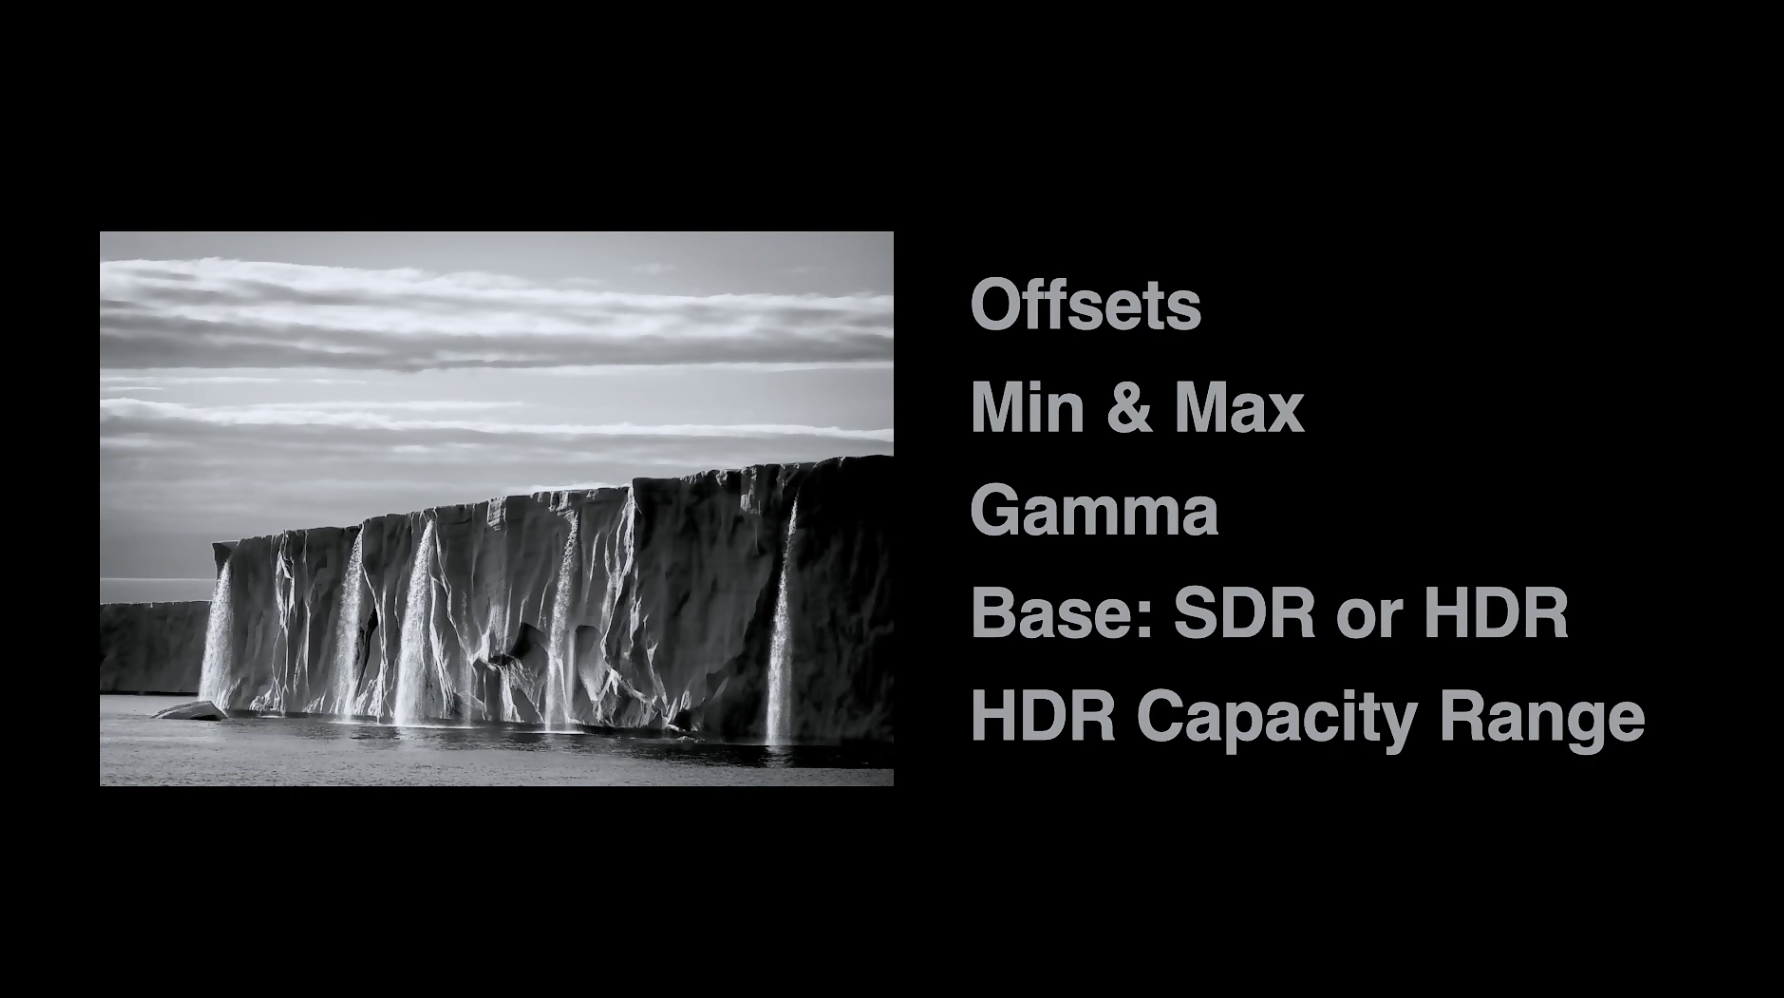
\includegraphics[width=0.65\textwidth]{gain_map_5.png}
    \caption{构成增益映射技术的核心元数据（Metadata）参数体系}
    \label{fig:metadata}
\end{figure}

增益映射并非简单的亮度提拉，其核心建立在线性光空间与对数空间的转换之上。理论上，像素增益即为 HDR 线性亮度与 SDR 线性亮度的商。为了防止纯黑像素导致的除零错误，以及暗部噪声造成的增益爆炸，规范引入了偏移常量 $offset_{hdr}$（或记为 $k_{hdr}$）和 $offset_{sdr}$（或记为 $k_{sdr}$），推荐默认值为 $0.015625$（即 $1/64$）：
\begin{equation}
pixel\_gain(x, y) = \frac{Y_{hdr}(x, y) + offset_{hdr}}{Y_{sdr}(x, y) + offset_{sdr}}
\end{equation}

由于人眼对光强度的对数感知特性，且 HDR 光比跨度极大，直接存储线性增益会导致严重量化误差。因此，编码器须提取增益极值（$map\_max\_log2$ 与 $map\_min\_log2$），将增益值转换至以 2 为底的对数空间，并进行归一化至 $[0.0, 1.0]$ 区间：
\begin{equation}
log\_recovery(x, y) = \frac{\log_2(pixel\_gain(x, y)) - map\_min\_log2}{map\_max\_log2 - map\_min\_log2}
\end{equation}
随后通过施加 Gamma 曲线以便在 8-bit 容器中高效存储：
\begin{equation}
recovery(x, y) = \left( \max(0.0, \min(1.0, log\_recovery(x, y))) \right)^{map\_gamma}
\end{equation}
在大多数实现中，$map\_gamma$ 被设为 1.0 以保持简洁可逆性。

\begin{figure}[H]
    \centering
    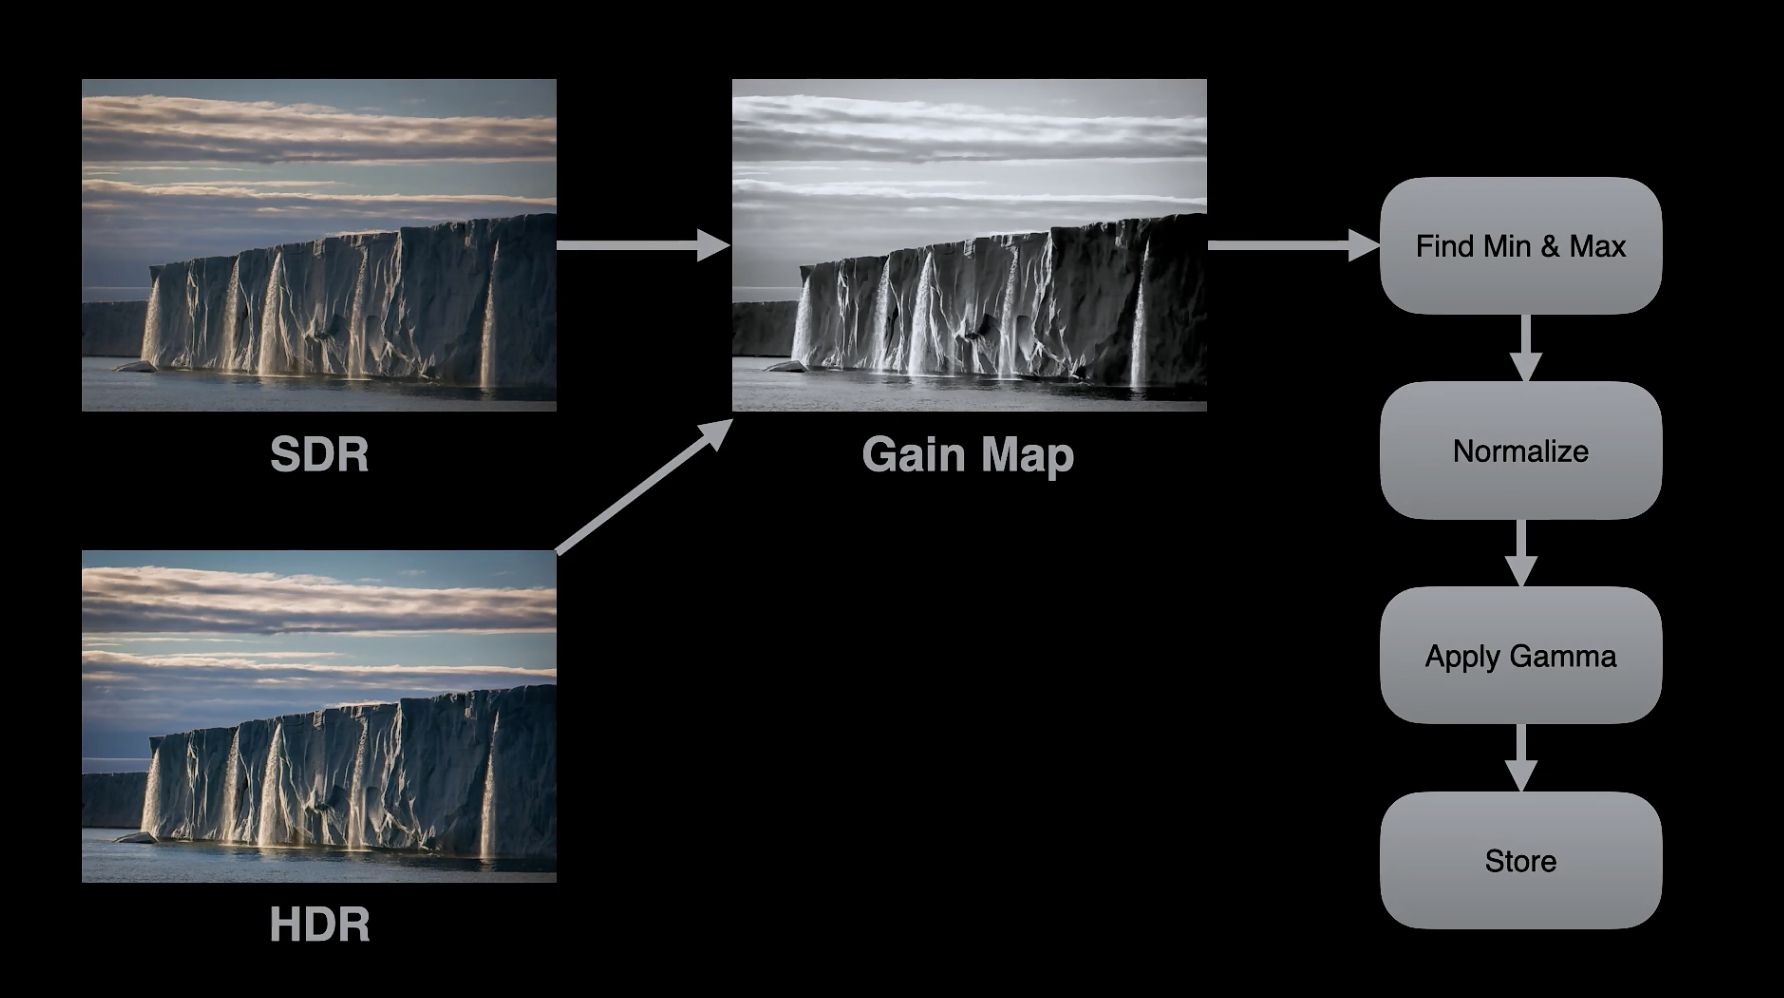
\includegraphics[width=0.65\textwidth]{gain_map_2.png}
    \caption{增益映射生成端（编码端）的数据处理管线}
    \label{fig:encoding_pipeline}
\end{figure}

\subsubsection{动态自适应重构与显示端渲染（与传统 EOTF 的关系）}

在传统的 HDR 视频流中，EOTF（如 PQ 曲线）会将传输的数字信号直接、刚性地映射为屏幕的绝对发光亮度。PQ 传递函数由 SMPTE ST 2084 定义，并纳入 ITU-R BT.2100 推荐标准\scite{1}\scite{2}。一旦文件要求 2000 尼特而屏幕仅支持 500 尼特，系统只能进行不可控的高光硬裁切或粗暴的色调映射。Gain Map 并没有取代 EOTF，而是在信号送入 EOTF 转换之前，插入了一个基于屏幕当前真实物理能力的\textbf{动态适配层}。

\begin{figure}[H]
    \centering
    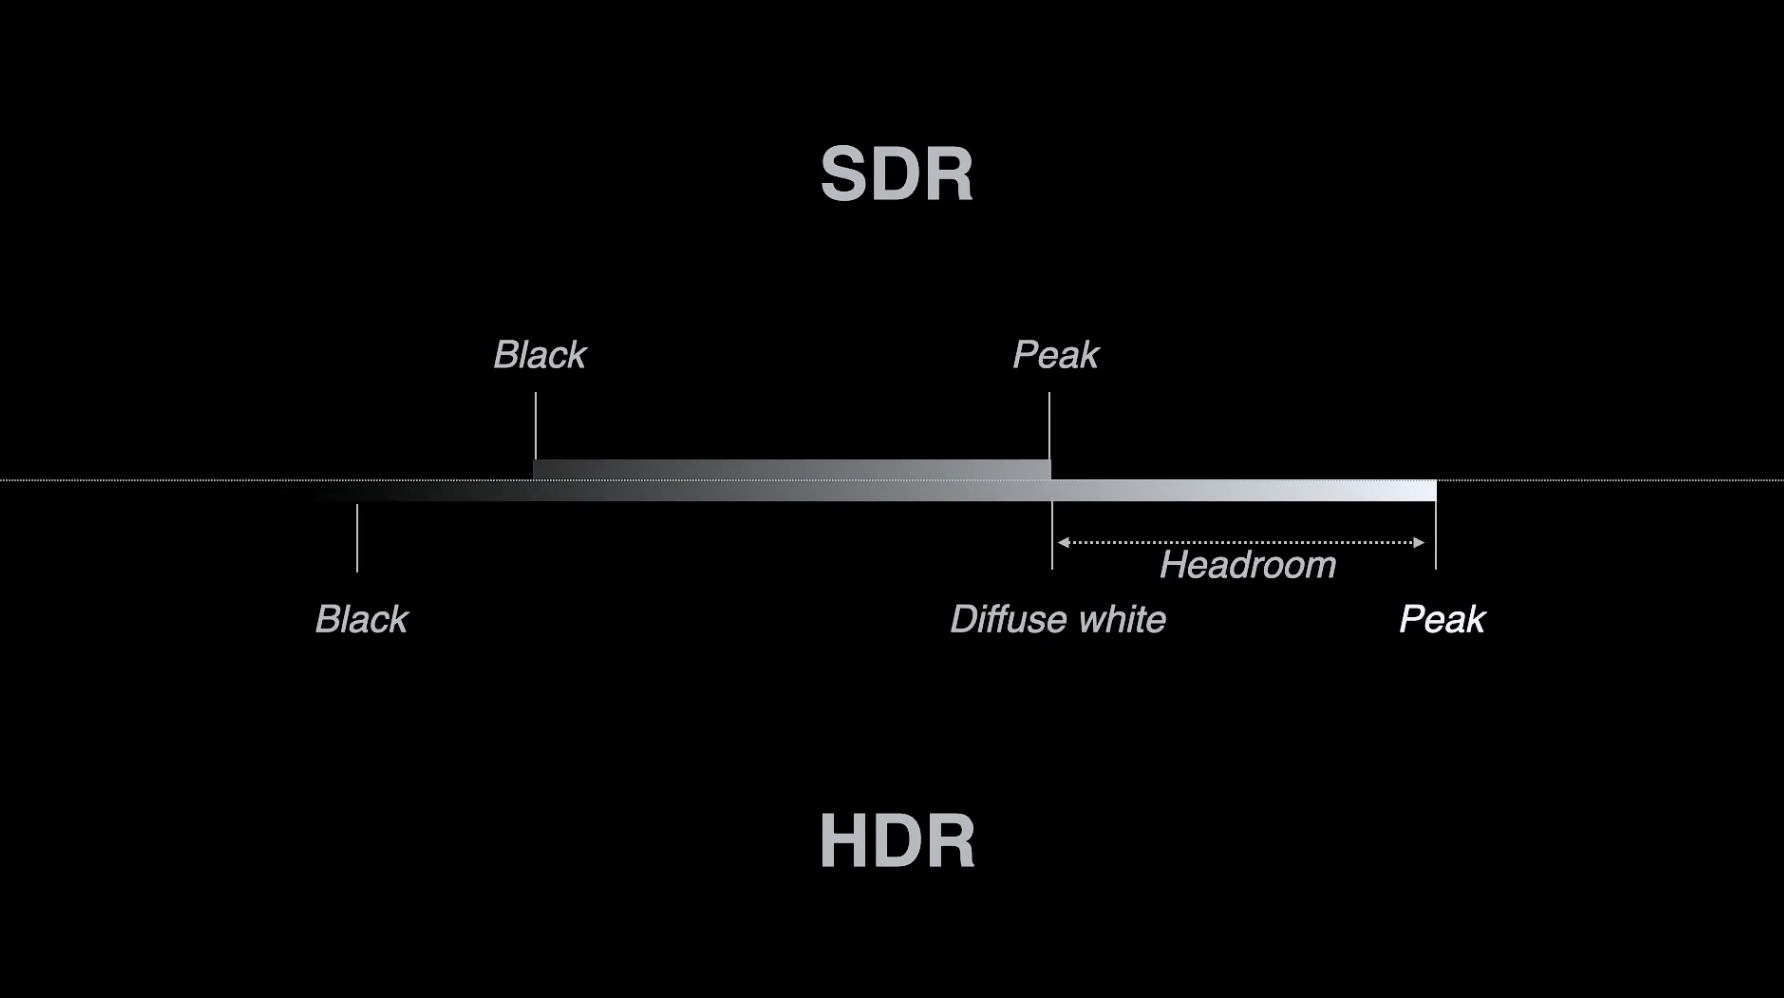
\includegraphics[width=0.7\textwidth]{gain_map_3.png}
    \caption{SDR 与 HDR 绝对亮度下的动态余量（Headroom）映射关系}
    \label{fig:headroom}
\end{figure}

系统首先查询屏幕真实的 HDR 余量，计算 $HDR_{capacity} = \log_2(HDR_{white} / SDR_{white})$，然后基于元数据设定的界限计算插值系数 $F$，进而得出最终用于合并运算的全局权重 $W$。当基础图像为 SDR 时，$W=F$；当基础图像为 HDR 时，$W=F-1$。

\begin{figure}[H]
    \centering
    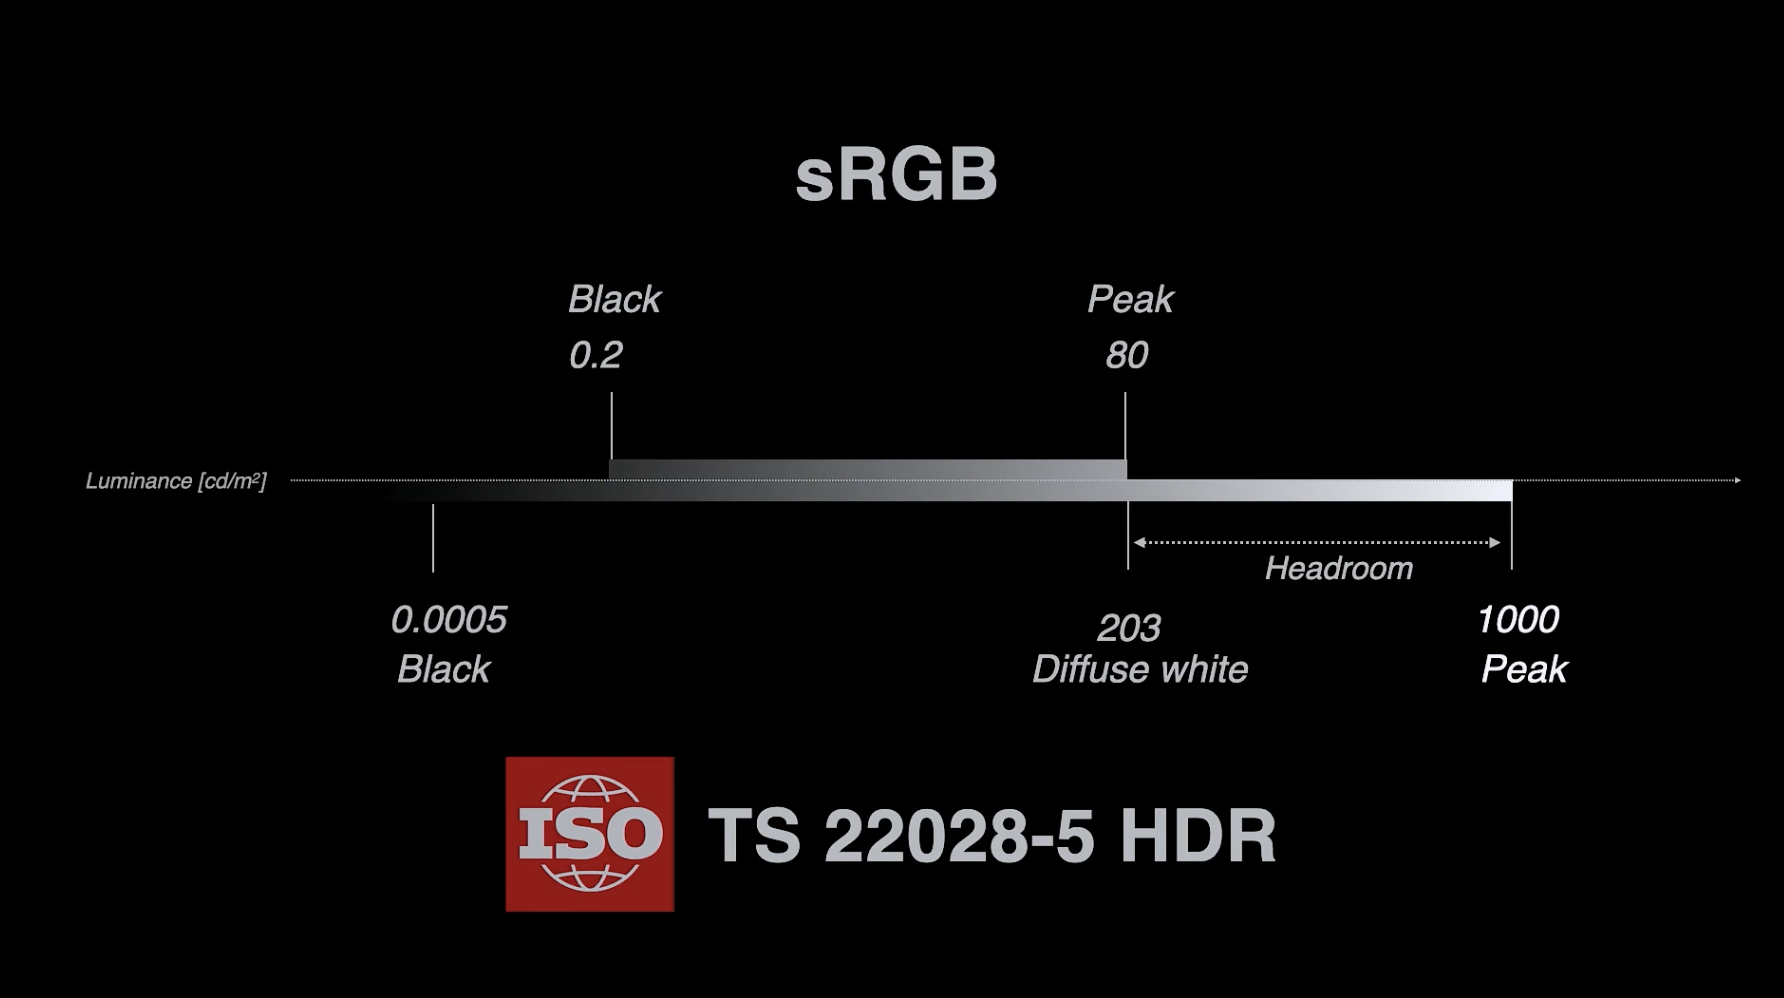
\includegraphics[width=0.7\textwidth]{gain_map_4.png}
    \caption{sRGB 与 ISO TS 22028-5 HDR 标准的光度量化区间对比}
    \label{fig:iso_hdr}
\end{figure}

最终在着色器渲染管线中，解码器提取增益图进行去伽马反归一化，乘上权重 $W$，然后通过指数还原算法与基础图像合并，计算出的完美自适应线性值才被送入底层的 EOTF 曲线去驱动屏幕发光。

\begin{lstlisting}[language=C, caption={Gain Map 渲染端重构着色器（Shader）核心逻辑}]
vec3 ApplyGainMap (image2d baseImage,
                   image2d gainMap,
                   vec2 position,
                   float w,             // weight for applying the gain map
                   vec3 gainMapMin,     // from gain map metadata
                   vec3 gainMapMax,     // from gain map metadata
                   vec3 gainMapGamma,   // from gain map metadata
                   vec3 offsetBase,     // from gain map metadata
                   vec3 offsetOther)    // from gain map metadata
{
    vec3 base = ReadImage (baseImage, position);
    vec3 gainMapEncoded = ReadImage (gainMap, position);
    vec3 gainMapLog2 = lerp (gainMapMin,
                             gainMapMax,
                             pow (gainMapEncoded, vec3 (1.0) / gainMapGamma));
    return ((base + offsetBase) * exp2 (gainMapLog2 * w)) - offsetOther;
}
\end{lstlisting}

值得注意的是，在 ISO 标准形成之前，Apple 在其操作系统的 AppKit 和 CoreImage 框架中采用了基于线性插值的另一种近似算法（Apple Adaptive HDR），将提取出的线性增益直接与 Headroom 进行线性插值：
$$
HDR_{rgb}(x, y) = SDR_{rgb}(x, y) \times \left( 1.0 + (headroom - 1.0) \times gainmap(x, y) \right)
$$
尽管这套早期算法计算更为简便，但在极端对比度下平滑度逊于对数空间插值。随着 ISO 21496-1 标准的普及，Apple 已在 iOS 18 和 macOS 15 中全面接纳了国际标准，将其命名为 Adaptive HDR，并与原生生态无缝融合\scite{16}。

\subsubsection{彩色（RGB）与单色增益映射的技术分野}
    
在工程实现中，增益映射表通常面临一个核心决策：使用单通道的灰度图（Monochrome）还是三通道的彩色图（RGB）？这一选择直接决定了图像在高光极值区域的色彩保真度。

为了最大化地节省存储空间并降低解码时的显存带宽压力，早期的多数手机厂商（甚至包括 Google 的默认实现）倾向于采用单通道黑白增益映射。在这种模式下，算法仅提取 HDR 图像与 SDR 图像的亮度（Luminance/Luma）通道，计算出一个全局标量增益矩阵：
\begin{equation}
Gain_{mono}(x, y) = \frac{Luma_{hdr}(x, y)}{Luma_{sdr}(x, y)}
\end{equation}
在解码时，这个单一的增益标量被同等地乘以 SDR 图像的红色、绿色和蓝色通道：
\begin{align}
R_{hdr} &= R_{sdr} \times Gain_{mono} \nonumber \\
G_{hdr} &= G_{sdr} \times Gain_{mono} \nonumber \\
B_{hdr} &= B_{sdr} \times Gain_{mono}
\end{align}

正如前文“硬件限制与色彩偏移的物理根源”小节所探讨的，当一张高动态范围场景（如鲜艳的夕阳、舞台强光）被压缩到 SDR 格式时，为了避免截断，SDR 生成算法通常已经改变了像素内 RGB 三通道的比例，导致高光区域出现褪色和色相偏移（例如原本纯红的晚霞在 SDR 中变成了偏黄的橙色）。
\textbf{黑白增益映射的致命缺陷在于：它只能恢复原始 HDR 图像的绝对亮度，但对 SDR 中已经发生偏移的 RGB 色彩比例无能为力}。当单色增益将那个“偏黄的橙色 SDR 像素”提亮 10 倍时，你得到的仅仅是一个极其刺眼的亮橙色像素，而根本无法还原出 HDR 原始捕获时的极致纯红色。在视觉观感上，这种高光色彩伪影会表现为高光泛白、色彩不自然、饱和度断层，严重破坏了数字艺术创作与自然摄影的真实感。

多通道彩色增益映射（RGB Gain Map）的引入，从根本上解决了这一物理与算法双重限制下的色偏难题。在 RGB 模式下，对数恢复映射不仅是一个二维矩阵，而是一个三维张量，编码器会为 Red、Green、Blue 三个通道分别计算并存储独立的增益值：
\begin{align}
pixel\_gain_R &= \frac{R_{hdr} + offset_{hdr}}{R_{sdr} + offset_{sdr}} \nonumber \\
pixel\_gain_G &= \frac{G_{hdr} + offset_{hdr}}{G_{sdr} + offset_{sdr}} \nonumber \\
pixel\_gain_B &= \frac{B_{hdr} + offset_{hdr}}{B_{sdr} + offset_{sdr}}
\end{align}

在解码重构 HDR 时，通过独立缩放每个通道，彩色增益映射能够在提亮的同时，精准地逆转 SDR 生成过程中的色调曲线压缩所带来的色彩畸变。即使 SDR 图像因为色调映射使得红色通道被过度压缩导致比例失衡，对应的红色通道增益（$pixel\_gain_R$）也会显著高于绿、蓝通道的增益。当各自相乘后，不仅恢复了绝对亮度，还完美还原了目标 HDR 像素真实的 R:G:B 比例与高光色彩。

在元数据层面，为了支撑彩色增益映射，XMP 命名空间或 ISO 二进制数据中的属性标签将不再是单一浮点数。例如，\texttt{GainMapMax}、\texttt{GainMapMin} 以及 \texttt{Gamma} 必须被定义为一个包含三个浮点数的数组（例如在 XML 中表现为 \texttt{<rdf:li>3.554440</rdf:li>}、\texttt{<rdf:li>3.473331</rdf:li>}、\texttt{<rdf:li>3.374647</rdf:li>}，分别对应 R、G、B 通道的最值）。

\begin{figure}[H]
    \centering
    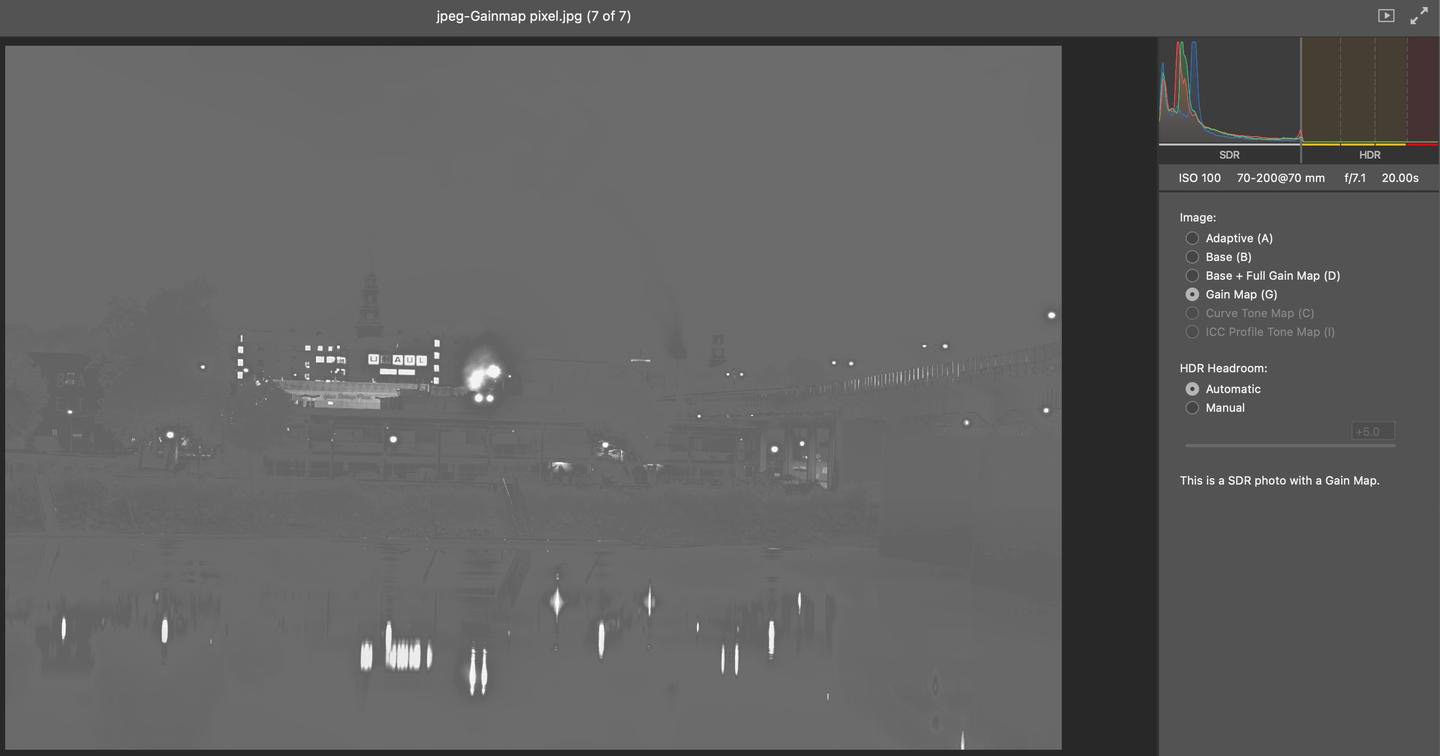
\includegraphics[width=0.8\textwidth]{gain_map_9.png}
    \caption{黑白（单色）增益映射数据可视化，仅包含全局亮度缩放信息}
    \label{fig:gain_map_gray}
\end{figure}

\begin{figure}[H]
    \centering
    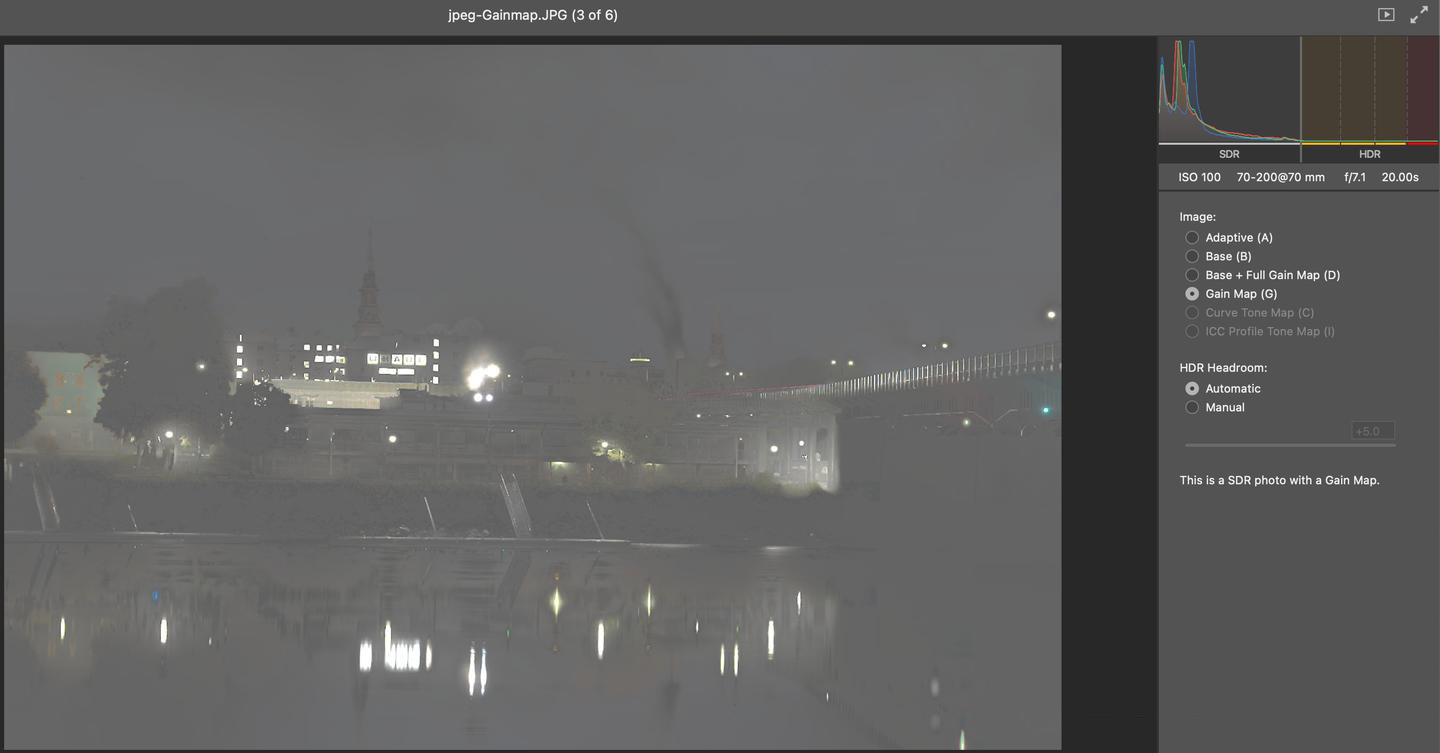
\includegraphics[width=0.8\textwidth]{gain_map_8.png}
    \caption{彩色（RGB）增益映射数据可视化，独立记录三通道的色彩提亮与纠偏信息}
    \label{fig:gain_map_color}
\end{figure}

\begin{table}[H]
\centering
\caption{黑白（单色）与彩色（RGB）增益映射的综合对比}
\begin{tabular}{@{} >{\raggedright\arraybackslash}p{3.5cm} >{\raggedright\arraybackslash}p{5.5cm} >{\raggedright\arraybackslash}p{5.5cm} @{}}
\toprule
\textbf{评估维度} & \textbf{黑白（单色）增益映射} & \textbf{彩色（RGB）增益映射} \\ \midrule
色彩还原能力 & 差。无法纠正 SDR 色调映射导致的高光色相漂移和饱和度丢失。 & 极高。完全保留 HDR 源文件的原始通道比例与高光色彩。 \\
元数据结构要求 & 单一标量值（GainMapMax 等属性为一个数字）。 & 浮点数序列数组（分别对应 R、G、B 通道）。 \\
存储开销与体积 & 极低。灰度图对总文件体积增加通常在 3\%–5\% 左右。 & 较高。存在 3 个色彩通道，压缩后体积约为单色图的 3 倍，但可通过降低分辨率缓解。 \\
终端计算复杂度 & 仅需一次标量乘法，极度适配移动设备及低功耗 GPU。 & 需对每个像素执行三次独立的通道浮点乘法，算力开销略大。 \\
最佳工程适用场景 & 缺乏高饱和高反差光源的日常场景；对体积极度敏感的应用。 & 夜景霓虹灯、夕阳、高对比人造光源、专业数字艺术分发。 \\ \bottomrule
\end{tabular}
\end{table}

此外，前沿研究开始探索放弃传统 DCT 图像格式存储增益图，转而使用轻量级的多层感知机（MLP）神经网络来编码增益映射。以 SDR 图像信息作为输入，针对性优化的微型 MLP 网络不仅在 HDR 重构表现上超越传统 JPEG 增益图，而且其模型权重仅需约 10 KB 的固定存储开销，为超高分辨率影像的精细 RGB 增益控制提供了革命性的低存储替代方案。

\subsubsection{元数据封装格式与多图片容器（MPF）规范}

增益映射技术的精妙之处在于对传统容器的复用，主要依赖于 CIPA DC-x 007-2009 Multi-Picture Format (MPF) 规范以及 XMP / APP2 标记段。在一个标准的 Ultra HDR JPEG 文件中，基础图像是第一个 JPEG 数据流，保证了向后兼容性；其头部包含标准的 APP1 XMP 数据段以及 MPF 索引，定义了文件中包含的图像总数和第二张辅助图像的绝对数据偏移量。在第一个 JPEG 结束标记之后，紧接着第二个 JPEG 数据流，即不可见的增益映射图像，其头部的 APP1 或 APP2 标记段中存储了至关重要的数学重构参数（如 \texttt{hdrgm:GainMap\_Min}、\texttt{hdrgm:GainMap\_Max} 等）。

\subsubsection{标准化演进：从 Adobe/Google 到 ISO 21496-1 的大一统架构}

在增益映射技术商业化初期，Apple（基于未公开 MakerNote 和自定公式的 Adaptive HDR）、Adobe（基于 \texttt{hdrgm} XMP 的规范）与 Google（基于 Adobe 规范衍生出的 Android 14 Ultra HDR）各自为政，导致跨平台 HDR 显示体验割裂。ISO 21496-1 标准的落地成为打通全平台生态的里程碑。相较于早期将元数据以纯文本 XML 存储在 APP1 中的方案，ISO 21496-1 规定核心元数据应以大端有理数的形式编码为紧凑的二进制结构，并直接嵌入到主图像与增益图的 APP2 标记段中。这一改变彻底消除了因十进制字符串格式化截断引入的精度损失，并在二进制层面提供了无可比拟的解析性能与文件鲁棒性。

\begin{table}[H]
\centering
\caption{早期 XMP 格式与 ISO 21496-1 二进制标准格式对比}
\begin{tabular}{@{} >{\raggedright\arraybackslash}p{3.5cm} >{\raggedright\arraybackslash}p{5cm} >{\raggedright\arraybackslash}p{5cm} @{}}
\toprule
\textbf{对比维度} & \textbf{早期 XMP（\texttt{hdrgm:} 命名空间）格式} & \textbf{ISO 21496-1 二进制标准格式} \\ \midrule
数据存储位置 & 主要位于增益图内部的 APP1 标记块中。 & 主图及增益图的 APP2 二进制块中（更深层耦合）。 \\
数据编码方式 & XML 格式化纯文本，属性值为浮点数字符串。 & 紧凑型二进制流，参数以大端有理数（分子/分母）形式存储。 \\
数学表示精度 & 较低。受限于十进制字符串序列化的截断误差。 & 极高。分数精确表示消除了浮点数舍入误差。 \\
生态兼容状态 & 早期过渡产物，目前作为兼容旧设备的后备方案。 & 国际共识标准，Android 15+、iOS 18+、macOS 15 及现代 Chrome 均原生解析。 \\
跨平台存活性 & 容易被常规 EXIF 清理工具或社交媒体后端压缩意外抹除。 & 深入数据流编解码层，难以被意外破坏，显著提升分发存活率。 \\ \bottomrule
\end{tabular}
\end{table}

目前，为保证生态平稳过渡，Android 15 系统底层 API、开源的 \texttt{libultra\_hdr}（v1.1 及以上）以及专业的后期软件普遍采用双重编码策略：既写入向后兼容的 XMP 文本标签，又写入前瞻性的 ISO 21496-1 APP2 二进制包。若解码器同时发现两种元数据，规范要求必须优先选用 ISO 21496-1 的参数进行 HDR 重构。

\subsubsection{手机计算摄影中的关键作用与跨设备生态适配}

\begin{figure}[H]
    \centering
    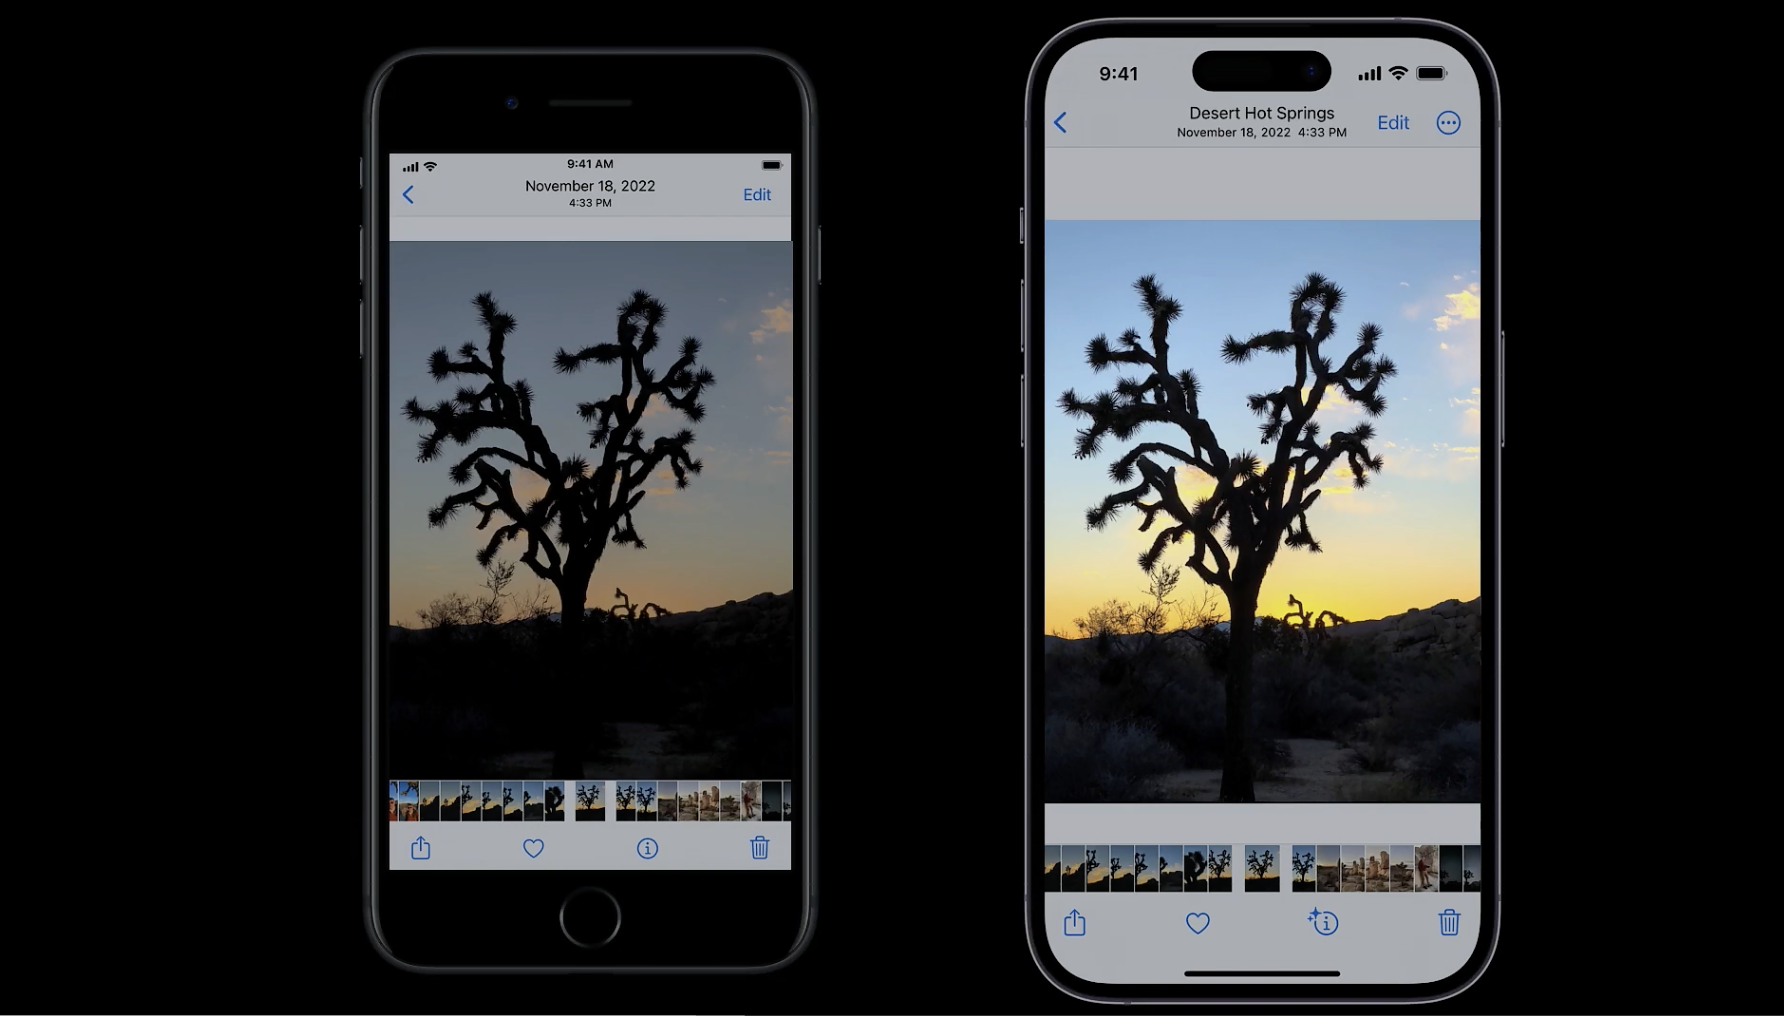
\includegraphics[width=0.65\textwidth]{gain_map_7.png}
    \caption{Gain Map 技术在不同物理显示能力的终端设备上的完美向下兼容}
    \label{fig:cross_device}
\end{figure}

在手机计算摄影中，Gain Map 之所以成为实现“超动态范围”显示的关键技术，是因为移动端生态（横跨无数 Android 与 iOS 终端）是全球硬件碎片化最严重的显示地带。手机计算摄影通过 Lofic 和多帧合成压榨出极高的宽容度，如果不加控制地直接输出为绝对亮度编码（如僵硬的 PQ HDR），在海量社交分享中将面临灾难性的观感断裂与高光塌陷。

伴随 \textbf{ISO 21496-1} 国际标准的落地，Apple、Adobe 与 Google 的规范走向了大一统\scite{16}。当前，基于 Chromium 的浏览器（Chrome、Edge 等）及 Apple Safari 均已实现对 ISO 21496-1 增益映射的全面原生解码，而在社交媒体分发层面，双重编码策略确保了新旧解析器均能正确触发 HDR 效果。通过这一套从底层数学到工业标准的彻底重构，影像分发不再受制于最低端屏幕的限制。在不支持 HDR 的旧手机上完美呈现 SDR 意图保底，而在最新的顶级 OLED 旗舰机上无缝解锁极致的峰值亮度，Gain Map 将创作者对高光的审美意图与不同屏幕的物理发光能力进行了彻底解耦，真正引领数字影像迈入了全终端自适应的时代。

% 参考文献
\newpage
% 为了参考文献的格式一致性，我们取消编号或者将 section 调整回原本的样式
\ctexset{section={number=\arabic{section},format=\centering\heiti\zihao{3},name={,}}} 
\phantomsection
\addcontentsline{toc}{section}{参考文献}
\begin{center}
    {\heiti\zihao{3} 参考文献}
\end{center}
\vspace{1em}
{\songti\zihao{-4}
\begin{enumerate}[label={[\arabic*]}]
    \item ITU-R BT.2100, \textit{Image parameter values for high dynamic range television for use in production and international programme exchange}. 2018.
    \item SMPTE ST 2084:2014, \textit{High Dynamic Range Electro-Optical Transfer Function of Mastering Reference Displays}.
    \item ARRI. \textit{ARRI LogC4 and ARRI Wide Gamut 4 White Paper}. 2023.
    \item ARRI. \textit{ARRI REVEAL Color Science White Paper}. 2023.
    \item Sony Corporation. \textit{S-Gamut3.Cine/S-Log3 and S-Gamut3/S-Log3 White Paper}. 2014.
    \item RED Digital Cinema. \textit{RED IPP2 Color Science: REDWideGamutRGB and Log3G10 White Paper}.
    \item 苹果公司. \textit{About Apple ProRes on iPhone — Apple Support}. 2024.
    \item Afifi, M. et al. \textit{Cross-Camera Convolutional Color Constancy}. Proceedings of the IEEE/CVF International Conference on Computer Vision, 2021.
    \item 程明，李翔. “面向移动端的 AI 白平衡算法研究”. 《影像科学与技术》. 2022, 40(3): 45-52.
    \item Tseng, T.-Y. et al. \textit{Time-Aware Auto White Balance in Mobile Photography}. ICCV 2025 / arXiv preprint, 2025.
    \item Bhayana, N. et al. \textit{Learning Camera-Agnostic White-Balance Preferences}. Proceedings of the IEEE/CVF Conference on Computer Vision and Pattern Recognition Workshops, 2024.
    \item ams OSRAM. \textit{Spectral Sensors for Automatic White Balancing (AWB) Enhance Color Consistency}. LEDinside Technical Report, 2026.
    \item Spectricity. \textit{S1 Multispectral Image Sensor — Product Overview}. 2023.
    \item OmniVision Technologies. \textit{OX03H10 Image Sensor with TheiaCel™ Technology Product Brief}. 2024.
    \item Google Android Developers. \textit{Ultra HDR Image Format Specification v1.2}. 2024.
    \item ISO 21496-1:2025, \textit{Gain map specification for HDR image interchange}. 2025.
    \item 张铭，刘振兴. 《数字电影摄影技术》. 北京：中国电影出版社，2020.
    \item Charles Poynton. \textit{Digital Video and HD: Algorithms and Interfaces}. Morgan Kaufmann, 2012.
    \item CIPA DC-x 007-2009. \textit{Multi-Picture Format (MPF) Specification}. Camera \& Imaging Products Association, 2009.
\end{enumerate}
}

\end{document}